% ------------------------------------------------------------------------
% ------------------------------------------------------------------------
% ICMC: Modelo de Trabalho Acadêmico (tese de doutorado, dissertação de
% mestrado e trabalhos monográficos em geral) em conformidade com 
% ABNT NBR 14724:2011: Informação e documentação - Trabalhos acadêmicos -
% Apresentação
% ------------------------------------------------------------------------
% ------------------------------------------------------------------------

% Opções: 
%   Qualificação         = qualificacao 
%   Curso                = doutorado/mestrado
%   Situação do trabalho = pre-defesa/pos-defesa (exceto para qualificação)
% -- opções do pacote babel --
% Idioma padrão = brazil
	%french,	    	% idioma adicional para hifenização
	%spanish,			% idioma adicional para hifenização
	%english,			% idioma adicional para hifenização
	%brazil				% o último idioma é o principal do documento
\documentclass[english]{packages/icmc}

% ---
% Pacotes Opcionais
% ---
\usepackage{rotating}           % Usado para rotacionar o texto
\usepackage[all,knot,arc,import,poly]{xy}   % Pacote para desenhos gráficos
% Este pacote pode conflitar com outros pacotes gráficos como o ``pictex''
% Então é necessário usar apenas um dos pacotes conflitantes


% ---
% Informações de dados para CAPA e FOLHA DE ROSTO
% ---
\titulo{Titulo do Trabalho de Conclusão de Curso }
\autor[de Moura, G. S.]{Gustavo de Moura Souza}
\orientador[Orientador:]{Prof. Dr.}{Claudio Fabiano Motta Toledo}
%\coorientador{Prof. Dr.}{Fulano de tal}
\curso{Computação}
\area{Sistemas Computacionais } % Área de concentração do trabalho
\data{01}{11}{2019} % Data do depósito
% ---


% ---
% RESUMOS
% ---

% Resumo em português
% conter no máximo 500 palavras
\textoresumo{
    Este trabalho é um breve modelo  para a escrita de monografias de qualificação, dissertações e teses utilizando o ambiente \LaTeX, de acordo com as normas exigidas pelo Instituto de Ciências Matemáticas e de Computação (ICMC), da Universidade de São Paulo (USP). Para a confecção deste modelo foi utilizado a última versão (1.9.2) do pacote de classes \textit{abnTeX2} que segue as normas da Associação Brasileira de Normas Técnicas. A elaboração de uma monografia, dissertação ou tese pode ser feita sobrescrevendo o conteúdo deste modelo. 
    }{Modelo, Monografia de qualificação, Dissertação, Tese, Latex}

% ---
% resumo em inglês
% ---
\textoresumo[english]{
    This paper is a brief model for writing qualification monographs, dissertations and thesis using \LaTeX environment, in accordance with the standards required by the Institute of Mathematics and Computer Sciences (ICMC), University of São Paulo (USP). For making this model, the latest version (1.9.2) \textit{abnTeX2} classes package was used. This package follow the rules of the Brazilian Association of Technical Standards. A drafting a monograph, dissertation or thesis can be done by overwriting the contents of this model.
    }{Template, Qualification monograph, Dissertation, Thesis, Latex}
    
% ---
% Configurações de aparência do PDF final
% ---
% alterando o aspecto da cor azul
\definecolor{blue}{RGB}{41,5,195}

% informações do PDF
\makeatletter
\hypersetup{
     	pagebackref=true,
		pdftitle={\@title}, 
		pdfauthor={\@author},
    	pdfsubject={\imprimirpreambulo},
	    pdfcreator={LaTeX with abnTeX2/ICMC-USP},
		pdfkeywords={\palavraschave}, 
		colorlinks=true,       		% false: boxed links; true: colored links
    	linkcolor=blue,          	% color of internal links
    	citecolor=blue,        		% color of links to bibliography
    	filecolor=magenta,      	% color of file links
		urlcolor=blue,
		bookmarksdepth=4
}
\makeatother
% --- 

% ----------------------------------------------------------
% ELEMENTOS PRÉ-TEXTUAIS
% ----------------------------------------------------------

% Inserir a ficha catalográfica
%\incluifichacatalografica[tex/fichaCatalografica.pdf]
\incluifichacatalografica


% Inserir folha de aprovação
%
% Isto é um exemplo de Folha de aprovação, elemento obrigatório da NBR
% 14724/2011 (seção 4.2.1.3). Você pode utilizar este modelo até a aprovação
% do trabalho. Após isso, substitua todo o conteúdo deste arquivo por uma
% imagem da página assinada pela banca com o comando abaixo:
%
% \includepdf{folhadeaprovacao_final.pdf}
%
\begin{folhadeaprovacao}

  \begin{center}
    {\ABNTEXchapterfont\large\imprimirautor}

    \vspace*{\fill}\vspace*{\fill}
    {\ABNTEXchapterfont\bfseries\Large\imprimirtitulo}
    \vspace*{\fill}
    
    \hspace{.45\textwidth}
    \begin{minipage}{.5\textwidth}
        \imprimirpreambulo
    \end{minipage}%
    \vspace*{\fill}
   \end{center}
    
   Trabalho aprovado. \imprimirlocal, 24 de novembro de 2012:

   \assinatura{\textbf{\imprimirorientador} \\ Orientador} 
   \assinatura{\textbf{Professor} \\ Convidado 1}
   \assinatura{\textbf{Professor} \\ Convidado 2}
   %\assinatura{\textbf{Professor} \\ Convidado 3}
   %\assinatura{\textbf{Professor} \\ Convidado 4}
      
   \begin{center}
    \vspace*{0.5cm}
    {\large\imprimirlocal}
    \par
    {\large\imprimirdata}
    \vspace*{1cm}
  \end{center}
  
\end{folhadeaprovacao}
% ---

% DEDICATÓRIA / AGRADECIMENTO / EPÍGRAFE
\textodedicatoria*{tex/pre-textual/dedicatoria}
\textoagradecimentos*{tex/pre-textual/agradecimentos}
\textoepigrafe*{tex/pre-textual/epigrafe}

% Inclui a lista de figuras
\incluilistadefiguras

% Inclui a lista de tabelas
\incluilistadetabelas

% Inclui a lista de quadros
\incluilistadequadros

% Inclui a lista de algoritmos
\incluilistadealgoritmos

% Inclui a lista de códigos
\incluilistadecodigos

% Inclui a lista de siglas e abreviaturas
\incluilistadesiglas

% Inclui a lista de símbolos
\incluilistadesimbolos

% ----
% Início do documento
% ----
\begin{document}

% ----------------------------------------------------------
% ELEMENTOS TEXTUAIS
% ----------------------------------------------------------
\textual

\chapter{Introdução}
\label{chapter:introducao}
\section{Motivação e Contextualização}

\section{Objetivos}

\section{Organização}



% Comando simples para exibir comandos Latex no texto
\newcommand{\comando}[1]{\textbf{$\backslash$#1}}

Este documento explica brevemente como trabalhar com a classe \LaTeX~\textit{icmc} para confeccionar trabalhos acadêmicos seguindo as normas da \sigla{ABNT}{Associação Brasileira de Normas Técnicas} e as \aspas{\textit{Diretrizes para apresentação de dissertações e teses da USP: documento eletrônico e impresso. Parte I (ABNT)}}, publicado pelo \sigla{SIBi}{Sistema Integrado de Bibliotecas} USP. O presente manual também atende as exigências prevista no regimento do Programa de Pós-graduação em \sigla{CCMC}{Ciências da Computação e Matemática Computacional} do \sigla{ICMC}{Instituto de Ciências Matemáticas e de Computação} da \sigla{USP}{Universidade de São Paulo}.


A classe \textit{icmc} foi construída com base na última versão da classe \textit{abntex2} e do pacote \textit{abntex2cite}. Portanto, este documento exemplifica a elaboração de trabalho
acadêmico (tese, dissertação e outros do gênero) produzido conforme a ABNT NBR
14724:2011 \textit{Informação e documentação - Trabalhos acadêmicos - Apresentação}.

Assim, é altamente recomendável que seja consultada a documentação do \textit{abntex2}\footnote{https://code.google.com/p/abntex2/downloads/list}. A classe \textit{abntex2} foi desenvolvida para facilitar a escrita de documentos seguindo as normas da ABNT no ambiente \LaTeX\;\cite{frasson:2005:classe_abnt}.

Todo o trabalho de pesquisa e ajustes da presente classe \LaTeX~\emph{icmc} foram feitos pelo aluno mestrado do Programa de Pós-graduação em Ciência da Computação e Matemática Computacional, Humberto Lidio Antonelli, durante a confecção da sua monografia de qualificação.

O requisito básico para utilização da classe \textit{icmc} é criar um documento desta classe com o comando
\comando{documentclass[@parameters]\{icmc\}} e ter, no diretório de trabalho, o arquivo \emph{icmc.cls} presente. Entretanto, recomenda-se fortemente manter a estrutura de diretório inicial fornecida por este modelo.

Os parâmetros possíveis utilizados pelo \comando{documentclass} são:
\begin{description}
\item[french, spanish, english, brazil] Adiciona o idioma para correta hifenização correta no documento. O último idioma declarado é o principal do documento. O valor padrão é \textbf{brazil}.
\end{description}



\chapter{Métodos, Técnicas e Tecnologias Utilizadas}
\label{chapter:metodos}




\chapter{Desenvolvimento}
\label{chapter:desenvolvimento}
\section{O Problema}

\section{Atividades Realizadas}

\section{Resultados}

\section{Dificuldades e Limitações}



\chapter{Conclusão}
\label{chapter:conclusao}
\input{tex/capitulos/conclusao}

\chapter{Instalando o abnTeX2}
\label{chapter:instalando-abntex}

A instalação do \emph{abnTeX2} varia de acordo com o sistema operacional empregado pelo usuário. Aqui serão apresentadas as formas de instalação nos sistemas mais utilizados atualmente no curso de ciência da computação do Câmpus Catalão, a saber: Linux (Ubuntu 12.04), Mac OS X e Windows 7

\section{Linux (Ubuntu 12.04)}

Se você já instalou o Tex Live via apt-get, basta seguir os seguintes comandos:

\begin{enumerate}

\item Baixe os arquivos de instalação do abnTeX2 (\url{http://code.google.com/p/abntex2/downloads/list}). Nesse link você também encontra a documentação e exemplos de uso.
\item Extraia o conteúdo do arquivo baixado na pasta texmf local, geralmente /usr/local/share/texmf. 
\item Em um Terminal: extraia o ZIP: \emph{unzip abntex2.tds.zip} em qualquer local;
\item copie o conteúdo extraído para o destino: \emph{cp abntex2/* /usr/local/share/texmf};
\item Em um Terminal digite: \emph{sudo texhash}
\item Pronto!
\end{enumerate}

\section{Mac OS}

Primeiramente, deve-se abrir o terminal do Mac que pode ser encontrado em Aplicativos/Utilitários - buscando pelo Finder.  E seguir os comandos abaixo:
\begin{enumerate}
\item Baixe os arquivos de instalação do abnTeX2 (\url{http://code.google.com/p/abntex2/downloads/list}). Nesse link você também encontra a documentação e exemplos de uso.
\item Extraia o conteúdo do arquivo baixado na pasta \emph{texmf} local, geralmente \emph{/usr/local/texlive/texmf-local}
\item Em um Terminal digite: \emph{sudo texhash}
\item Pronto!
\end{enumerate}
 
 \section{Windows 7}

\subsection{Instalar/atualizar pelo Package Manager (recomendado)}

Geralmente o abnTeX2 é baixado e instalado automaticamente pelo MiKTeX quando o usuário compila pela primeira vez um dos modelos do abnTeX2. Porém, caso isso não ocorra, siga os passos seguintes:

\begin{enumerate}
\item Clique em Iniciar/Start -> Todos os Programas/All Programs -> MiKTeX -> Package Manager;
\item Clique em Repository / Synchronize;
\item Clique com o botão direito sobre \emph{abntex2} na lista e selecione Install (ou Update, caso já esteja instalado);
\item Pronto!
\end{enumerate}

\subsection{Instalar/atualizar manualmente}

Você apenas precisará utilizar a instalação manual no caso de:

\begin{enumerate}
\item o abnTeX2 não estar na lista de pacotes do MiKTeX por alguma razão;
\item você não poder utilizar uma conexão com a Internet no momento da instalação;
\item a versão do abnTeX2 no MiKTeX estar desatualizada em relação à versão disponível no CTAN.
\end{enumerate}
Em qualquer caso, lembre-se de remover uma eventual instalação anterior do abnTeX2 . Se houver instalado pelo Package Manager, remova o abnTeX2 também por ele.

Passos para instalação manual do abnTeX2 no MiKTeX:

\begin{enumerate}
\item Baixe os arquivos de instalação do abnTeX2 (abntex2.tds-vX.X.zip). Nesse link você também encontra a documentação e exemplos de uso.
\item Extraia o conteúdo do arquivo baixado em uma pasta qualquer;
\item Você pode criar uma pasta abntex2, por exemplo, em $C:\backslash abntex2\backslash$;
\item Consulte http://www.tex.ac.uk/cgi-bin/texfaq2html?label=install-where para outras informações;
\item Clique em Iniciar/Start -> Todos os Programas/All Programs -> MiKTeX -> Settings;
\item Na aba Roots, adicione o diretório recém criado;
\item Na aba General, clique em Refresh FNDB, OU, se preferir, em um Terminal digite initexmf --update-fndb;
\item Pronto!
\end{enumerate}

\chapter{Orientações Gerais}
\label{chapter:orientacoes-gerais}


\section{Codificação dos arquivos: UTF8}

A codificação de todos os arquivos do \abnTeX\ é \texttt{UTF8}. É necessário que
você utilize a mesma codificação nos documentos que escrever, inclusive nos
arquivos de base bibliográficas |.bib|.



\section{Inclusão de outros arquivos}\label{sec-include}

É uma boa prática dividir o seu documento em diversos arquivos, e não
apenas escrever tudo em um único. Esse recurso foi utilizado neste
documento. Para incluir diferentes arquivos em um arquivo principal,
de modo que cada arquivo incluído fique em uma página diferente, utilize o
comando:

\begin{verbatim}
   \include{documento-a-ser-incluido}      % sem a extensão .tex
\end{verbatim}

Para incluir documentos sem quebra de páginas, utilize:

\begin{verbatim}
   \input{documento-a-ser-incluido}      % sem a extensão .tex
\end{verbatim}



%\section{Remissões internas}

%Ao nomear a \autoref{tab-nivinv} e a \autoref{fig_circulo}, apresentamos um exemplo de remissão interna, que também pode ser feita quando indicamos o \autoref{cap_exemplos}, que tem o nome \emph{\nameref{cap_exemplos}}. O número do capítulo indicado é \ref{cap_exemplos}, que se inicia à \autopageref{cap_exemplos}\footnote{O número da página de uma remissão pode ser obtida também assim: \pageref{cap_exemplos}.}.
%Veja a \autoref{sec-divisoes} para outros exemplos de remissões internas entre seções, subseções e subsubseções.

%O código usado para produzir o texto desta seção é:

%\begin{verbatim}
%Ao nomear a \autoref{tab-nivinv} e a \autoref{fig_circulo}, apresentamos um
%exemplo de remissão interna, que também pode ser feita quando indicamos o
%\autoref{cap_exemplos}, que tem o nome \emph{\nameref{cap_exemplos}}. 
%O número
%do capítulo indicado é \ref{cap_exemplos}, que se inicia à
%\autopageref{cap_exemplos}\footnote{O número da página de uma remissão pode ser
%obtida também assim:
%\pageref{cap_exemplos}.}.
%Veja a \autoref{sec-divisoes} para outros exemplos de remissões internas entre
%seções, subseções e subsubseções.
%\end{verbatim}



\section{Consulte o manual da classe \textsf{abntex2}}

Consulte o manual da classe \textsf{abntex2} \cite{abntex2classe} para uma
referência completa das macros e ambientes disponíveis. 

Além disso, o manual possui informações adicionais sobre as normas ABNT
observadas pelo \abnTeX\ e considerações sobre eventuais requisitos específicos
não atendidos, como o caso da \citeonline[seção 5.2.2]{NBR14724:2011}, que
especifica o espaçamento entre os capítulos e o início do texto, regra
propositalmente não atendida pelo presente modelo.



\section{Precisa de ajuda?}

Consulte a FAQ com perguntas frequentes e comuns no portal do \abnTeX:
\url{https://code.google.com/p/abntex2/wiki/FAQ}.

Inscreva-se no grupo de usuários \LaTeX:
\url{http://groups.google.com/group/latex-br}, tire suas dúvidas e ajude
outros usuários.

Participe também do grupo de desenvolvedores do \abnTeX:
\url{http://groups.google.com/group/abntex2} e faça sua contribuição à
ferramenta.



\section{Você pode ajudar?}

Sua contribuição é muito importante! Você pode ajudar na divulgação, no
desenvolvimento e de várias outras formas. Veja como contribuir com o \abnTeX\
em \url{https://code.google.com/p/abntex2/wiki/ComoContribuir}.

\chapter{Configuração dos Elementos Pré-Textuais}
\label{chapter:config-pre-textual}
A configuração de diversas opções e principalmente dos elementos pré-textuais é realizada com comandos específicos inseridos antes do comando \comando{begin\{document\}}. As informações do documento são configuradas através dos comandos:

\begin{description}

 \item[\comando{titulo\{T\}}] Título do trabalho (substitua T pelo título do trabalho);

 \item[\comando{autor[REF]\{N\}}] Nome do autor do trabalho (onde REF é como o nome do autor é referenciado e N é o nome do autor);

 \item[\comando{orientador\{T\}\{O\}}] Nome do professor orientador do trabalho. Caso seja uma orientadora pode ser usado o comando \comando{orientador[Orientadora:]\{T\}\{O\}} (sendo que T é a titulação do professor e O é o nome do orientador);

 \item[\comando{coorientador\{T\}\{C\}}] Nome do professor coorientador do trabalho. Caso seja uma coorientadora pode ser usado um comando análogo a definição de orientadora  empregando o comando \comando{coorientador[Coorientadora:]\{T\}\{C\}}(sendo que T é a titulação do professor e C é o nome do orientador);

 
 \item[\comando{curso\{EP\}\{NP\}}] Dados do programa de Pós-Graduação (onde EP é a especialidade que será atribuída ao pós-graduando e NP é o nome do programa de pós-graduação.  Exemplo: \comando{curso\{Ciências -- Ciências de Computação e Matemática Computacional\}\{Ciências de Computação e Matemática Computacional\}};
 
 \item[\comando{data\{dia\}\{mês\}\{ano\}}] Configuração da data do depósito do documento;

 \item[\comando{textoresumo\{TR\}\{PC\}}] Texto do resumo (TR) e palavras-chave (PC) do documento sendo separadas por vírgula. Se o idioma do resumo for diferente do declarado no documento, pode ser usado o comando \comando{textoresumo[L]\{TR\}\{PC\}} (sendo que L é a linguagem do resumo).
 
\end{description}

As opções seguintes correspondem também as configurações dos elementos pré-textuais, porém seu uso é opcional: 

\begin{description}

 \item[\comando{textodedicatoria\{TD\}}] Texto referente a dedicatória do trabalho (TD). Caso o texto esteja em um arquivo separado (recomendado para que o projeto fique modularizado e os documentos mais limpo), deve utilizar o comando \comando{textodedicatoria*\{ARQ\}}, em que ARQ é o nome do arquivo, incluindo o caminho do diretório se necessário;

 \item[\comando{textoagradecimentos\{TA\}}] Texto referente aos agradecimentos do trabalho (TA). Caso o texto esteja em um arquivo separado (recomendado para que o projeto fique modularizado e os documentos mais limpo), deve utilizar o comando \comando{textoagradecimentos*\{ARQ\}}, em que ARQ é o nome do arquivo, incluindo o caminho do diretório se necessário;

 \item[\comando{incluilistadefiguras}] Comando para inclusão da lista de figuras. Deve-se utilizar este comando somente quando o ambiente \textbf{figure} for utilizado no documento;
 
 \item[\comando{incluilistadetabelas}] Comando para inclusão da lista de tabelas. Deve-se utilizar este comando somente quando o ambiente \textbf{table} for utilizado no documento;
  
 \item[\comando{incluilistadequadros}] Comando para inclusão da lista de quadros. Deve-se utilizar este comando somente quando o ambiente \textbf{quadro} for utilizado no documento;
   
 \item[\comando{incluilistadealgoritmos}] Comando para inclusão da lista de algoritmos. Deve-se utilizar este comando somente quando o ambiente \textbf{algoritmo} for utilizado no documento;
    
 \item[\comando{incluilistadecodigos}] Comando para inclusão da lista de figuras. Deve-se utilizar este comando somente quando o ambiente \textbf{codigo} for utilizado no documento;
 
 \item[\comando{incluilistadesiglas}] Comando para inclusão da lista de siglas e abreviaturas. Deve-se utilizar este comando somente quando existirem siglas e abreviaturas no documento, com a utilização do comando \comando{sigla\{S\}\{DS\}} ou \comando{sigla*\{S\}\{DS\}};

 \item[\comando{incluilistadesimbolos}] Comando para inclusão da lista de símbolos. Deve-se utilizar este comando somente quando existirem símbolos no documento, com a utilização do comando \comando{simbolo\{S\}\{DS\}}.
 
\end{description}

\chapter{Corpos Flutuantes}
\label{chapter:corpos-flutuantes}

Corpos flutuantes são elementos não textuais, como figuras e tabelas, que complementam as informações do texto. Neste capítulo são expostos breves exemplos dos corpos flutuantes disponíveis na classe \textit{icmc}.

Na \autoref{secao:figuras} é mostrado como inserir figuras, a \autoref{secao:tabelas_e_quadros} explica como incluir tabelas e quadros, a \autoref{secao:algoritmos_e_codigos} demostra como trabalhar com algoritmos e códigos-fonte e a \autoref{secao:outros-ambientes} explica como definir outros ambientes para serem utilizados, como para gráficos e diagramas.

\section{Figuras}
\label{secao:figuras}

A inserção de figuras é realizada normalmente através do comando \comando{begin\{figure\}}. Na \autoref{figura:logomarca_usp} é exibida a logomarca da USP com o pacote \textit{graphicx}. Já a \autoref{figura:exemplo_grafo} mostra um exemplo de grafo com o pacote \textit{xy}. De acordo com as normas ABNT a lista de figuras é um elemento opcional do documento, para incluí-la é preciso inserir o comando \comando{incluidelistafiguras} antes do início do documento.

Observe que, segundo a \citeonline[seções 4.2.1.10 e 5.8]{NBR14724:2011}, as
ilustrações devem sempre ter numeração contínua e única em todo o documento. Além disso, deve ser incorporado ao corpo flutuante do tipo figura, além da legenda, a fonte de onde esta foi extraída. Se a figura foi confeccionada pelo próprio autor, deve se colocar "Elaborada pelo autor".

\begin{citacao}
Qualquer que seja o tipo de ilustração, sua identificação aparece na parte
superior, precedida da palavra designativa (desenho, esquema, fluxograma,
fotografia, gráfico, mapa, organograma, planta, quadro, retrato, figura,
imagem, entre outros), seguida de seu número de ordem de ocorrência no texto,
em algarismos arábicos, travessão e do respectivo título. Após a ilustração, na
parte inferior, indicar a fonte consultada (elemento obrigatório, mesmo que
seja produção do próprio autor), legenda, notas e outras informações
necessárias à sua compreensão (se houver). A ilustração deve ser citada no
texto e inserida o mais próximo possível do trecho a que se
refere. \cite[seções 5.8]{NBR14724:2011}
\end{citacao}

\begin{figure}[htb]
 \caption{Logomarca da USP}
 \label{figura:logomarca_usp}
 \centering
 
\includegraphics[scale=0.3]{images/usp-logo}
 \fdireta{usp:logo}
\end{figure}


\begin{figure}[htb]
\caption{Exemplo de grafo}
\label{figura:exemplo_grafo}
\centering
\begin{scriptsize}
$$
\xymatrix@R20pt@C10pt{
 & & & & vr \ar[dlll] \ar[dl] \ar[d] \ar[dr] \ar[drr] \ar[drrr] & & & \\
 & (a_3, b_2, c_1) \ar[d]^{\varphi_2} \ar[dl]_{\varphi_1} & & (a_3, b_2, c_2) \ar[d]^{\varphi_2} \ar[dl]_{\varphi_1} & (a_1, b_1, c_1) & (a_1, b_1, c_2) & (a_1, b_2, c_1) & (a_1, b_2, c_2) \\
 (a_2, b_2, c_1) \ar[dr]_{\varphi_3} & (a_3, b_1, c_1) \ar[d]^{\varphi_1} & (a_2, b_2, c_2) \ar[dr]_{\varphi_3} & (a_3, b_1, c_2) \ar[d]^{\varphi_1} & & & & \\
& (a_2, b_1, c_1)  & & (a_2, b_1, c_2) & & & & \\
}
$$
\end{scriptsize}
\fautor
\end{figure}

A classe \textit{icmc} traz algum comando que auxiliam na inserção da legenda, para utilizá-los basta substituir o \comando{fonte\{\}} por um dos seguintes comando conforme necessário:

\begin{description}

 \item[\comando{fautor}] Insere o texto \aspas{Elaborada pelo autor} como fonte da figura;

 \item[\comando{fadaptada[INF]\{REF\}}] Insere um texto informando que a figura foi adaptada de alguma referência bibliográfica (REF). INF refere-se ao local específico de onde a imagem foi extraída, como por exemplo o número da página. Além disso, INF é um parâmetro opcional e pode receber qualquer cadeia de texto;

 \item[\comando{fdireta[INF]\{REF\}}] Insere um texto informando que a figura próvem diretamente de alguma referência bibliográfica (REF). INF refere-se ao local específico de onde a imagem foi extraída, como por exemplo o número da página. Além disso, INF é um parâmetro opcional e pode receber qualquer cadeia de texto;
 
 \item[\comando{fdadospesquisa}] Insere o texto \aspas{Dados da pesquisa.} como fonte da figura;
 
\end{description}



\section{Tabelas e Quadros}
\label{secao:tabelas_e_quadros}

A inserção de tabelas e quadros é feita de forma semelhante a inserção de figuras, porém são utilizados os ambientes \textit{table} e \textit{quadro}. A principal diferença entre tabelas e quadros, de acordo com \citeonline{silveira:2006:manual_tcc}, é que as tabelas são destinadas para informações numéricas e os quadros são mais adequados para informações textuais. Em geral, as tabelas devem estar padronizadas conforme o padrão do
\citeonline{ibge1993} requerido pelas normas da ABNT para documentos técnicos e
acadêmicos.

Como exemplos foram inseridas a \autoref{tabela:lista_produtos} que exibe uma de lista de produtos (construída em \LaTeX) e a Tabela \autoref{tabela:populacao_america_sul} que mostra a população dos países da América do Sul (construída segundo o padrão do IBGE). Foi inserido também o \autoref{quadro:editores_texto_livres} com alguns editores que podem ser usados para se trabalhar com \LaTeX para demonstrar a inserção de quadros.

 A lista de tabelas também é um elemento opcional que pode ser incluída com o comando \comando{incluidelistatabelas} antes do início do documento. O mesmo acontece com a lista de quadros que pode ser incluída com o comando \comando{incluidelistaquadros}.

\begin{table}[htb]
\centering
\caption{Lista de produtos}
\label{tabela:lista_produtos}
\begin{tabularx}{\textwidth}{X|l|r|r|r} \hline
Produto      & Unidade & Preço (R\$) & Quantidade & Total (R\$) \\ \hline
Arroz        & Kg      & 2,00        & 550        & 1.100,00    \\
Óleo de Soja & L       & 2,50        & 500        & 750,00      \\
Açucar       & Kg      & 3,00        & 100        & 300,00      \\ \hline
\end{tabularx}
\fdadospesquisa
\end{table}

\begin{table}[htb]
\IBGEtab{%
  \caption{População dos países da América do Sul} \label{tabela:populacao_america_sul}
}{%
\begin{tabular}{r|p{3cm}|r}        
\toprule
Código  & País            & População   \\ \midrule \midrule
1       & Brasil          & ~~~~~~191.480.630 \\ \midrule 
2       & Argentina       &  39.934.100 \\ \midrule 
3       & Colômbia        &  46.741.100 \\ \midrule 
4       & Paraguai        &   9.694.200 \\ \midrule 
5       & Uruguai         &   3.350.500 \\ \midrule 
6       & Peru            &  28.221.500 \\ \midrule 
7       & Equador         &  13.481.200 \\ \midrule 
8       & Bolívia         &   9.694.200 \\ \midrule 
9       & Venezuela       &  28.121.700 \\ \midrule 
10      & Chile           &  16.803.000 \\ \bottomrule
\end{tabular}
}{%
  \fdireta{wikipedia:2011:america_sul}%
  \nota{Esta é uma nota, que diz que os dados são baseados na
  regressão linear.}%
  \nota[Anotações]{Uma anotação adicional, que pode ser seguida de várias
  outras, porém são opcionais.}%
  }
\end{table}

\begin{quadro}[htb]
\caption{Editores de Texto Livres}
\label{quadro:editores_texto_livres}
\centering
\begin{tabular}{|l|l|r|}        \hline
Editor     & Multiplataforma & Específico para Latex \\ \hline
Kwriter    & Sim             & Não                   \\
Texmaker   & Sim             & Sim                   \\
Kile       & Sim             & Sim                   \\
Geany      & Sim             & Não                   \\ \hline
\end{tabular}
\end{quadro}

\section{Algoritmos e Códigos}
\label{secao:algoritmos_e_codigos}

Além dos corpos flutuantes convencionais para inserir figuras (\comando{begin\{figure\}}) e tabelas (\comando{begin\{table\}}), a classe \textit{icmc} possui mais dois tipos de corpos flutuantes um para algoritmos (\comando{begin\{algoritmo\}}) e outro para códigos-fonte (\comando{begin\{codigo\}}). A utilização de um ou de outro fica a critério do usuário. Como exemplo temos o \autoref{algoritmo:mdc1} que calcula o máximo divisor comum entre dois números e os Códigos-fonte \ref{codigo:notas_alunos} e \ref{codigo:metodo_leitura} que são uma consulta na \sigla{SQL}{\textit{Structured Query Language}} e uma sobrotina em \textit{Java}.

%\begin{algoritmo}[htb]
\begin{algoritmo}
%\begin{algorithmic}[1]
\caption{Algoritmo para cálculo de máximo divisor comum MDC($n_1$,$n_2$)}
\label{algoritmo:mdc1}

 \KwIn{Dois números inteiros ($n_1, n_2$)}
 \If(\tcp*[f]{Garante que o maior número seja $n_1$}){$n_2 > n_1$}
   {troca valores de $n_1$ e $n_2$}
 \Repeat{$r > 0$}{
    $r \leftarrow$ resto da divisão de $n_1$ por $n_2$
    $n_1 \leftarrow n_2$
    $n_2 \leftarrow r$
 }
 \Return $n_1$
%\end{algorithmic}
\end{algoritmo}
%\end{algoritmo}

%\begin{codigo}[htb]
%\caption{Consulta SQL}
%\label{codigo:notas_alunos}
%\hrule
\begin{codigo}[caption = {Consulta SQL}, label={codigo:notas_alunos},language=SQL, breaklines=true]
SELECT a.nome_aluno AS aluno,
       d.nome_disciplina AS disciplina,
       m.nota AS nota
FROM aluno AS a,
     disciplina AS d,
     matriculado AS m
WHERE a.id_aluno = m.id_aluno
  AND d.id_disciplina = m.id_disciplina
ORDER BY a.nome_aluno, d.nome_disciplina;
\end{codigo}
%\end{codigo}

%\begin{codigo}[htb]
%\caption{Subrotina para obter uma entrada do usuário}
%\label{codigo:metodo_leitura}
%\hrule
\begin{codigo}[caption={Subrotina para obter uma entrada do usuário}, label={codigo:metodo_leitura}, language=Java, breaklines=true]
public static String Leitura(){
    BufferedReader reader = new BufferedReader(new InputStreamReader(System.in));
    try {
        return reader.readLine(); // Lê uma linha pelo teclado
    } catch (IOException e) {
        e.printStackTrace();
        return "";
    }
}
\end{codigo}
%\end{codigo}

Existem diversos outros pacotes disponíveis para escrever algoritmos e códigos. Nos exemplos anteriormente foram utilizados o pacote \textit{algorithm} para definição do ambiente algoritmo e \textit{listings} para a definição do ambiente de código-fonte. O pacote \textit{algorithm} é usado para escrever algoritmos em alto nível \cite{janos:2005:algpseudocode}. Já o pacote \textit{listings} serve para escrever os códigos em diversas linguagens de programação \cite{moses:2006:listings}.

Caso sejam utilizados os ambientes de algoritmos e código podem ser incluídos os comandos \comando{incluidelistaalgoritmos} e \comando{incluidelistacodigos} antes do \comando{begin\{document\}} para que a lista de algoritmos e a lista de código sejam criadas.


\section{Ambientes Matemáticos}

A classe \textit{icmc} provê os seguintes ambientes matemáticos:
\begin{itemize}
 \item Teoremas (\comando{begin\{teorema\}[\ ]} ... \comando{begin\{teorema\}});
 \item Proposição (\comando{begin\{proposicao\}[\ ]} ... \comando{begin\{proposicao\}});
 \item Lema (\comando{begin\{lema\}[\ ]} ... \comando{begin\{lema\}});
 \item Corolário (\comando{begin\{corolario\}[\ ]} ... \comando{begin\{corolario\}});
 \item Exemplo (\comando{begin\{exemplo\}[\ ]} ... \comando{begin\{exemplo\}});
 \item Observação (\comando{begin\{observacao\}[\ ]} ... \comando{begin\{observacao\}});
 \item Definição (\comando{begin\{definicao\}[\ ]} ... \comando{begin\{definicao\}});
 \item demonstracao (\comando{begin\{demonstracao\}[\ ]} ... \comando{begin\{demonstracao\}}).
\end{itemize}

Abaixo temos um exemplo de proposição com sua demonstração:
\begin{proposicao}
 Sejam $a$ e $b$ reais, tais que $0<a<b$. Então $a^2<b^2$.
\end{proposicao}
\begin{demonstracao}
 Pela hipótese concluímos que $(b+a)>0$ e $(b-a)>0$.

Como $b^2-a^2=(b+a)(b-a)$ concluímos que $b^2-a^2>0$, ou seja, $a^2<b^2$.
\end{demonstracao}

Neste documento tratamos brevemente apenas dos ambientes mencionados anteriormente. Contudo, para escrever expressões matemáticas complexas é preciso estudar uma documentação mais específica como em \citeonline{cassagojr:1997:amslatex}.

Alguns dos ambientes matemáticos da classe \textit{icmc} podem ser usados também para outras finalidades como exemplos e definições.


\section{Definição de outros ambientes}
\label{secao:outros-ambientes}

O classe \textit{icmc} permite a criação de outros ambientes, além dos citados nas seções anteriores, caso seja necessário. Isso é possível graças a extensão da classe \textit{abntex}. O \autoref{codigo:novo-ambiente} deve ser inserido antes do início do documento para criação de um ambiente para gráficos. Para definição de outros ambientes, basta seguir o modelo.


\begin{codigo}[caption={Definição do ambiente \textbf{grafico}}, label={codigo:novo-ambiente}, language=Tex, breaklines=true]
\makeatletter

% Novo list of (listings) para GRÁFICOS --------------------------
\newcommand{\graficoname}{Gráfico}
\newcommand{\graficorefname}{Gráfico}
\newcommand{\listofgraficosname}{Lista de gráficos}

\addto\captionsenglish{% ingles
    %% adjusts names from abnTeX2
    \newcommand{\graficoname}{Graph}
    \newcommand{\graficorefname}{Graph}
    \newcommand{\listofgraficosname}{List of graphs}
}

\newfloat[chapter]{grafico}{logr}{\graficoname}
\newlistof{listofgraficos}{logr}{\listgraficoname}
\newlistentry{grafico}{logr}{0}

% configurações para atender às regras da ABNT
\renewcommand{\thegrafico}{\thechapter.\@arabic\c@grafico}
\setfloatadjustment{grafico}{\centering}
\renewcommand{\cftgraficoname}{\graficoname\space}
\renewcommand*{\cftgraficoaftersnum}{\hfill\textendash\hfill}
% ----------------------------------------------------------------

\makeatother
\end{codigo}

A utilização do novo ambiente no texto segue conforme o \autoref{codigo:usar-novo-ambiente}.

\begin{codigo}[caption={Como usar o ambiente \textbf{grafico}}, label={codigo:usar-novo-ambiente}, language=Tex, breaklines=true]
\begin{grafico}[htb]
\caption{Caption do gráfico}
\label{gra:modelo}
Este é o conteúdo do gráfico.
\end{grafico}
\end{codigo}

Comandos como \comando{autoref\{gra:modelo\}} funcionam normalmente.

Para imprimir a "Lista de gráficos" no documento, insira o \autoref{codigo:lista-novo-ambiente} na classe \textit{icmc}, de modo que ele seja impresso após a "Lista de ilustrações". O código deve ser inserido após a linha 1244.


\begin{codigo}[caption={Código para inserir lista de gráficos}, label={codigo:lista-novo-ambiente}, language=Tex, breaklines=true]
% ---
% inserir lista de gráficos
% ---
\pdfbookmark[0]{\listofgraficosname}{logr}
\listofgraficos*
\cleardoublepage
% ---
\end{codigo}

\chapter{Listas}
\label{chapter:listas}
\section{Abreviaturas e Siglas}

A classe \textit{icmc} implementa a criação da lista de abreviaturas e siglas com o pacote \textit{nomencl}. A inserção de abreviaturas e siglas na lista é realizada com o comando \comando{sigla\{A\}\{B\}}, onde \textit{A} é a sigla e \textit{B} é o nome por extenso. Para se gerar a lista de siglas na parte pre-textual é preciso incluir o comando \comando{incluidelistasiglas} antes do início do documento. Além disto, a compilação do documento deve conter o comando \textit{makeindex} após duas compilações com o \textit{pdflatex}. Por exemplo, supondo que o documento principal tenha o nome de \textit{monografia}, podemos usar a seguinte sequência de comandos:
\begin{verbatim}
pdflatex monografia.tex
pdflatex monografia.tex
makeindex monografia.nlo -s nomencl.ist -o monografia.nls
pdflatex monografia.tex
\end{verbatim}

No Capítulo \ref{chapter:ferramentas-uteis} serão apresentadas algumas ferramentas que podem facilitar o processo de compilação do documento.

\section{Símbolos}

A definição de símbolos é semelhante a definição de siglas, porém deve ser usado o comando \comando{simbolo\{S\}\{DS\}}, onde \textit{S} é o símbolo e \textit{DS} é a descrição do símbolo. Como exemplo definimos os símbolos \simbolo{\mathbb{X}}{Variável X}$\mathbb{X}$ e \simbolo{\mathsf{I\!R}}{Conjunto dos números reais}$\mathsf{I\!R}$. Para incluir a lista de símbolos, basta usar o comando \comando{incluidelistasimbolos} antes do início do documento.


\chapter{Ferramentas Úteis}
\label{chapter:ferramentas-uteis}
Existem diversas ferramentas para se trabalhar com \LaTeX. Duas ferramentas que merecem destaque são o editor \textit{Texmaker} exibido na Figura \ref{figura:texmaker} e o gerenciador de referências \textit{JabRef} mostrado na Figura \ref{figura:jabref}. Ambas ferramentas são livres e multiplataforma.

\begin{figure}[htb]
\caption{Tela do Texmaker}
 \label{figura:texmaker}
 \centering
 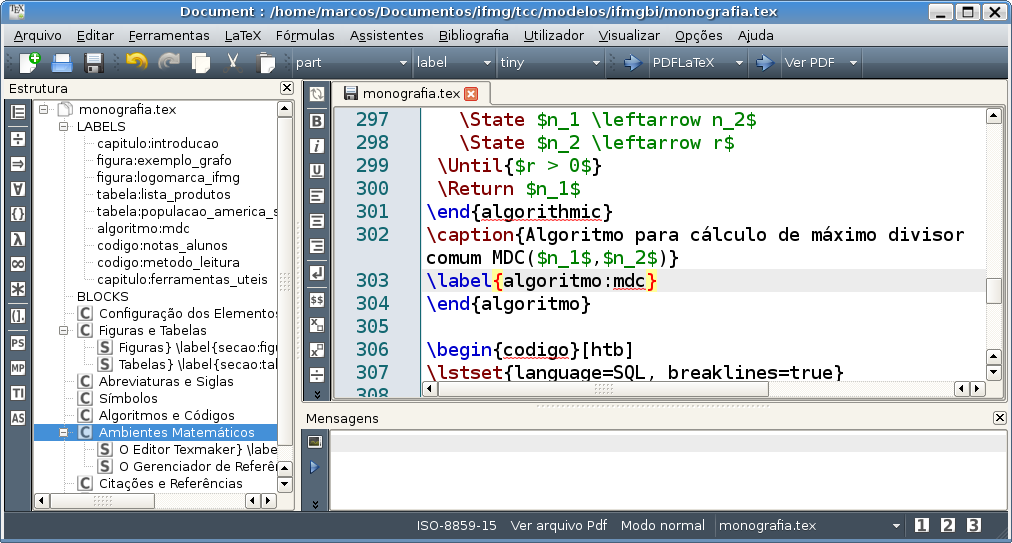
\includegraphics[width=\textwidth]{texmaker}
 \legend{Fonte: o autor.}
\end{figure}

\begin{figure}[htb]
 \caption{Tela do JabRef}
 \label{figura:jabref}
 \centering
 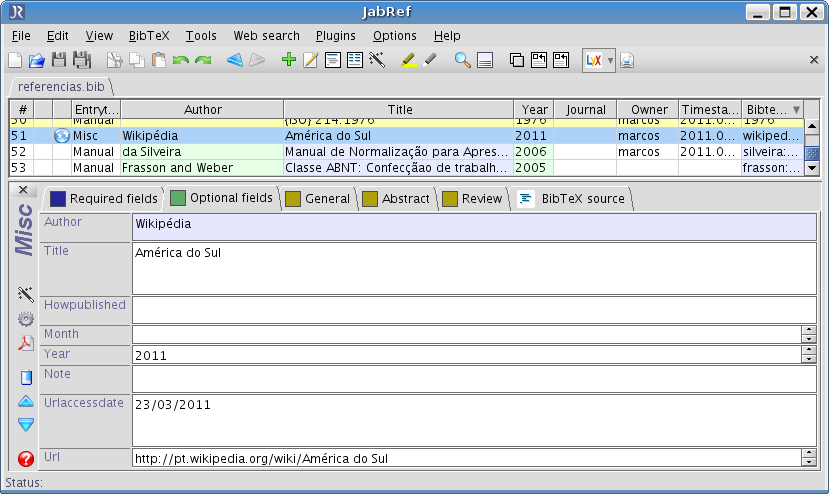
\includegraphics[width=\textwidth]{jabref}
\legend{Fonte: o autor.}
\end{figure}

O Texmaker pode ser obitido em \url{www.xm1math.net/texmaker} e o JabRef pode ser obtido em \url{jabref.sourceforge.ne}. É importante ressaltar que o Texmaker é apenas um editor, para compilar os documentos é necessário um ambiente \LaTeX instalado. Os ambientes Latex mais populares são o Texlive (\url{www.tug.org/texlive}) e o MiKTex (\url{miktex.org}).

\chapter{Citações e Referências}
\label{chapter:citacoes}
Em documentos acadêmicos podem existir citações diretas e citações indiretas. As citações indiretas são feitas quando se reescreve uma referência consultada. Nas citações indiretas há duas formatações possíveis dependendo de como ocorre a citação no texto. Quando o autor é mencionado explicitamente  deve ser usado o comando \comando{citeonline\{\}}, nas demais situações é usado o comando \comando{cite\{\}}. No quadro \ref{figura:citacao_indireta_explicita} encontrasse um  exemplo de uso do comando \comando{citeonline\{\}}.

\begin{quadro}[htb]
\caption{Exemplo de citação indireta explícita} \label{figura:citacao_indireta_explicita}
\hrulefill

\lstset{language=Tex, breaklines=true}
\begin{lstlisting}
Segundo \citeonline{silveira:2006}, o trabalho de conclusão de curso deve seguir as normas da ABNT.
\end{lstlisting}

\hrulefill

Segundo \citeonline{silveira:2006:manual_tcc}, o trabalho de conclusão de curso deve seguir as normas da ABNT.

\hrulefill

%\legend{Fonte: o autor.}
\end{quadro}

Para especificar a página consultada na referência é preciso acrescentá-la entre colchetes com os comandos \comando{cite[página]\{\}} ou \comando{citeonline[página]\{\}}. No quadro \ref{figura:citacao_indireta_pagina} é mostrado um exemplo de citação com página específica.

\begin{quadro}[htb]
\caption{Exemplo de citação indireta não explícita} \label{figura:citacao_indireta_pagina}
\hrulefill

\lstset{language=Tex, breaklines=true}
\begin{lstlisting}
A folha de aprovação é um elemento obrigatório na monografia de projeto final de curso trabalho de conclusão de curso.  \cite[p.~10]{silveira:2006}.
\end{lstlisting}

\hrulefill

A folha de aprovação é um elemento obrigatório no trabalho de conclusão de curso.  \cite[p.~10]{silveira:2006:manual_tcc}.

\hrulefill

\end{quadro}

As citações diretas acontecem quando o texto de uma referência é transcrito literalmente. As citações diretas são curtas (até três linhas) são inseridas no texto entre aspas duplas. Conforme exemplo no quadro \ref{figura:citacao_direta_curta}.

\begin{quadro}[htb]
\caption{Exemplo de citação direta curta}
\label{figura:citacao_direta_curta}
\hrulefill

\lstset{language=Tex, breaklines=true}
\begin{lstlisting}
``Os quadros, ao contrário das tabelas, apresentam dados textuais e devem localizar-se o mais próximo do texto a que se referem'' \cite[p.~25]{silveira:2006}.
\end{lstlisting}

\hrulefill

``Os quadros, ao contrário das tabelas, apresentam dados textuais e devem localizar-se o mais próximo do texto a que se referem'' \cite[p.~25]{silveira:2006:manual_tcc}.

\hrulefill
\end{quadro}

As citações longas (com mais de 3 linhas) podem ser inseridas via \comando{begin\{citacao\}} conforme quadro \ref{figura:citacao_direta_longa}.

\begin{quadro}[htb]
\caption{Exemplo de citação direta longa}
\label{figura:citacao_direta_longa}
\hrulefill

\lstset{language=Tex, breaklines=true}
\begin{lstlisting}
\begin{citacao}
Síntese final do trabalho, a conclusão constitui-se de uma resposta à hipótese enunciada na introdução. O autor manifestará seu ponto de vista sobre os resultados obtidos e sobre o alcance dos mesmos. Não se permite a inclusão de dados novos nesse capítulo nem citações ou interpretações de outros autores \cite[p.~25]{silveira:2006}.
\end{citacao}
\end{lstlisting}

\hrulefill

\begin{citacao}
Síntese final do trabalho, a conclusão constitui-se de uma resposta à hipótese enunciada na introdução. O autor manifestará seu ponto de vista sobre os resultados obtidos e sobre o alcance dos mesmos. Não se permite a inclusão de dados novos nesse capítulo nem citações ou interpretações de outros autores \cite[p.~25]{silveira:2006:manual_tcc}.
\end{citacao}

\hrulefill

\end{quadro}


% ---
% Finaliza a parte no bookmark do PDF, para que se inicie o bookmark na raiz
% ---
\bookmarksetup{startatroot}% 
% ---

% ----------------------------------------------------------
% ELEMENTOS PÓS-TEXTUAIS
% ----------------------------------------------------------
\postextual

% ----------------------------------------------------------
% Referências bibliográficas
% ----------------------------------------------------------
\bibliography{references}

% ---------------------------------------------------------------------
% GLOSSÁRIO
% ---------------------------------------------------------------------

% Arquivo que contém as definições que vão aparecer no glossário
\newword{1}{Agentes de usuário}{qualquer \textit{software} que recupera, processa e facilita a interação do usuário final com o conteúdo  Web. Como exemplo desses agentes, podem ser citados navegadores, reprodutores multimídia e tecnologias assistivas} 

\newword{2}{ATAG}{\textit{Authoring Tool Accessibility Guidelines} ou Diretrizes de acessibilidade para ferramentas de autoria. É um conjunto de diretrizes para desenvolvedores de qualquer ferramenta de criação para Web, como: simples editores HTML, ferramentas para exportar conteúdo para Web, ferramentas multimídia e sistemas de gerenciamento de conteúdo}

\newword{3}{DOM}{\textit{Document Object Model} ou Modelo de Objetos de Documentos. É uma especificação do W3C para organizar objetos de um documento em que se pode, dinamicamente, alterar e editar sua estrutura, conteúdo e estilo}

\newword{4}{Javascript}{é uma linguagem de \textit{script} para desenvolvimento de certos tratamentos 
que ocorrem lado do cliente, geralmente o navegador Web. Ela é utilizada geralmente quando 
é inconveniente ou impossível para o servidor para fazer esse tratamento}

\newword{5}{Stakeholder}{qualquer pessoa ou grupo, que legitima as ações de uma organização. É formado pelos funcionários da empresa, gestores, gerentes, proprietários, fornecedores, clientes, o Estado, credores, sindicatos e diversas outras pessoas ou empresas que estejam relacionadas com uma determinada ação ou projeto.}

\newword{6}{Tag}{ou etiqueta, é uma palavra-chave ou termo associado com uma informação que a descreve. Em linguagens de marcação, como o HTML, consistem em breves instruções, tendo uma marca de início e outra de fim para que o navegador possa mostrar a renderização da página}

\newword{7}{Tecnologia assistiva}{Conjunto de técnicas, aparelhos, instrumentos, produtos e procedimentos que visam auxiliar a mobilidade, percepção e utilização do meio ambiente e dos elementos por pessoas com deficiência	}

\newword{8}{UAAG}{\textit{User Agent Accessibility Guidelines} ou Diretrizes de acessibilidade para agentes de usuário. Conjuntos de diretrizes para desenvolvedores de agentes de usuário (por exemplo: navegadores e reprodutores de mídia) com a finalidade de fazer com que tais agentes permitam sua utilização adequada por pessoas com algum tipo de deficiência}

\newword{9}{W3C}{\textit{World Wide Web Consortium}. É um consórcio internacional formado por empresas, órgãos governamentais e organizações independentes que visa desenvolver padrões para a criação e a interpretação de conteúdos da Web}

\newword{10}{WAI}{\textit{Web Accessibility Initiative} ou Iniciativa de Acessibilidade na Web. É a iniciativa do W3C no que tange a desenvolver estratégias, diretrizes e outros recursos, a fim de que as informações presentes na Web sejam acessíveis para pessoas com ou sem deficiência}

\newword{11}{WCAG}{\textit{Web Content Accessibility Guidelines} ou Diretrizes de Acessibilidade para Conteúdo Web. É um conjunto de diretrizes criado pelo W3C para auxílio na elaboração de conteúdo acessível, que atualmente está em sua versão 2.0 desde 2008.}

\newword{12}{WYSIWYG}{``What You See Is What You Get''  ou ``O que você vê é o que você obtém''.  Recurso tem por objetivo permitir que um documento, enquanto manipulado na tela, tenha a mesma aparência de sua utilização, usualmente sendo considerada final. Isso facilita para o desenvolvedor que pode trabalhar visualizando a aparência do documento sem precisar salvar em vários momentos e abrir em um \textit{software} separado de visualização}

\newword{13}{Desenho universal}{concepção de produtos, ambientes, programas e serviços a serem usados, na maior medida possível, por todas as pessoas, sem necessidade de adaptação ou projeto específico. O desenho universal não excluirá as ajudas técnicas para grupos específicos de pessoas com deficiência, quando necessárias}

\newword{14}{Mobilidade reduzida}{dificuldade permanente ou temporária que uma pessoa tem para se movimentar, gerando redução efetiva da mobilidade, flexibilidade, coordenação motora e percepção}

\newword{15}{Pessoas com deficiência}{aquelas que têm impedimentos de longo prazo de natureza física, mental, intelectual ou sensorial, os quais, em interação com diversas barreiras, podem obstruir sua participação plena e efetiva na sociedade em igualdades de condições com as demais pessoas. Atualmente chegou-se a um consenso quanto à utilização da expressão ``pessoa com deficiência'' em todas as suas manifestações orais ou escritas, em lugar de termos como ``deficiente'', ``pessoa portadora de deficiência'', ``pessoa com necessidades especiais'' e ``portador de necessidades especiais''}

\newword{16}{Framework}{é uma abstração que une códigos comuns entre vários projetos de \textit{software} provendo uma funcionalidade genérica. \textit{Frameworks} são projetados com a intenção de facilitar o desenvolvimento de \textit{software}, habilitando designers e programadores a gastarem mais tempo determinando as exigências do \textit{software} do que com detalhes de baixo nível do sistema}

\newword{17}{Dojo Toolkit}{é uma biblioteca em JavaScript, de código fonte aberto, projetado para facilitar o rápido desenvolvimento de interfaces ricas}

\newword{18}{Meta-tag}{Uma etiqueta HTML identificando o conteúdo de um \textit{website}. Informações comumente encontradas na meta-tag incluem: direitos autorais, palavras-chave para ferramentas de busca e descrições da formatação da página}

\newword{19}{DOCTYPE}{\textit{Document Type Definition} ou Definição do tipo de documento. Indica para o navegador e para outros meios qual a especificação de código utilizar. O DOCTYPE não é uma \textit{tag} do HTML, mas uma instrução para que o navegador tenha informações sobre qual versão de código a marcação foi escrita}

\newword{20}{Template}{é um documento sem conteúdo, com apenas a apresentação visual (apenas cabeçalhos por exemplo) e instruções sobre onde e qual tipo de conteúdo deve entrar a cada parcela da apresentação}

\newword{21}{Padrões de projeto}{ou \textit{Design Pattern}, descreve uma solução geral reutilizável para um problema recorrente no desenvolvimento de sistemas de \textit{software} orientados a objetos. Não é um código final, é uma descrição ou modelo de como resolver o problema do qual trata, que pode ser usada em muitas situações diferentes}

\newword{22}{e-MAG}{Modelo de Acessibilidade de Governo Eletrônico. Consiste em um conjunto de recomendações a ser considerado para que o processo de acessibilidade dos sítios e portais do governo brasileiro seja conduzido de forma padronizada e de fácil implementação}

\newword{23}{Web}{Sinônimo mais conhecido de \textit{World Wide Web} (WWW). É a interface gráfica da Internet que torna os serviços disponíveis totalmente transparentes para o usuário e ainda possibilita a manipulação multimídia da informação}

% Comando para incluir todas as definições do arquivo glossario.tex
\glsaddall
% Impressão do glossário
\printglossaries

% ----------------------------------------------------------
% Apêndices
% ----------------------------------------------------------

% ---
% Inicia os apêndices
% ---
\begin{apendicesenv}

    \chapter{Documento Básico Usando a Classe icmc}
    \label{chapter:documento-basico}
    
\begin{codigo}[caption={Exemplo de um documento básico}, label={codigo:documento-basico}, language=Tex, breaklines=true]
% Documento utilizando a classe ufgcac
% Opções: 
%   Qualificação         = qualificacao 
%   Curso                = doutorado/mestrado
%   Situação do trabalho = pre-defesa/pos-defesa (exceto para qualificação)
% -- opções do pacote babel --
% Idioma padrão = brazil
	%french,	    % idioma adicional para hifenização
	%spanish,			% idioma adicional para hifenização
	%english,			% idioma adicional para hifenização
	%brazil				% o último idioma é o principal do documento
\ documentclass[doutorado, spanish, english, brazil]{packages/icmc}

% Título do trabalho
\titulo{Título da Monografia}

% Nome do autor
\autor[Abreviação]{Nome completo do autor}

% Define o local
\local{São Carlos -- SP}

% Data do depósito
\data{18}{12}{2012}

% Nome do Orientador
\orientador[Orientador:]{Titulação do orientador}{Nome completo do Orientador}

% Nome do Coorientador (caso não exista basta remover)
\coorientador[Coorientador:]{Titulação do coorientador}{Nome completo do Coorientador}
% Se coorientadora troque Coorientador: por Coorientadora: dentro do colchetes

% Define o nome da instituição
\instituicao{Instituto de Ciências Matemáticas e de Computação (ICMC/USP)}

% Especiolidade e Nome do programa de Pós-graduação
\curso[Ciências -- Ciências de Computação e Matemática Computacional]{Ciências de Computação e Matemática Computacional}
% O valor entre colchetes é opcional

% Resumo
\textoresumo[Idioma]{
Texto do resumo do trabalho.
}{Lista de palavras-chave separada por virgulas}


% Início do documento
\begin{document}

\chapter{Introdução}

Capítulo de Introdução

\chapter{Desenvolvimento}

Capítulo de Desenvolvimento

\chapter{Conclusão}

Capítulo de conclusão

% Nome do arquivo com as referências bibliográficas
\bibliography{referencias}

\end{document}

\end{codigo}

\end{apendicesenv}
% ---


% ----------------------------------------------------------
% Anexos
% ----------------------------------------------------------

% ---
% Inicia os anexos
% ---
\begin{anexosenv}

    \chapter{Páginas Interessantes na Internet} 
    \label{chapter:paginas-interessantes}
    \begin{description}
 \item[\url{http://www.tex-br.org}]: Página em português com diversos tutoriais e referências interessantes sobre \LaTeX;
 \item[\url{http://en.wikibooks.org/wiki/LaTeX}]: Livro em formato \textit{wiki} gratuito sobre \LaTeX;
 \item[\url{http://tobi.oetiker.ch/lshort/lshort.pdf}]: Ótimo tutorial sobre \LaTeX (possui versão em português \url{http://alfarrabio.di.uminho.pt/~albie/lshort/ptlshort.pdf}, mas a versão em inglês é a mais atual);
 \item[\url{http://code.google.com/p/abntex2/}]: Página do abnTeX2, grupo que desenvolve os pacotes e classes em \LaTeX para as normas da ABNT, nos quais a classe \textit{icmc} foi baseada;
\item[\url{ http://www.rexlab.ufsc.br:8080/more/index.jsp}]: Página do Mecanismo On-line para Referências  (MORE) desenvolvido pela UFSC.
 \end{description}

\end{anexosenv}
% ---

\end{document}